\chapter{802.15.4 Standard}
\label{chap:802154standard}

Work-group \ac{IEEE} 802.15 was formed to elaborate a standard for the \ac{WPAN}. Inside this work-group, the Task Group 4 
deals with the low binary rate ones, \ac{LR-WPAN}. Last standard revision was approved in 2006 with the name of: ``Wireless 
Medium Access Control (\ac{MAC}) and Physical Layer (\ac{PHY}) Specifications for Low-Rate Wireless Personal Area Networks (\acp{WPAN})'' 
\cite{IEEE802.15.4-2006}.

As it can be observed in the title, the standard defines only the Physical Layer and the \ac{MAC} Layer. Using this basis, 
this work will build the Network, Transport and Application Layers to define the entire network behavior according to the proposed 
High Configurable Protocol.

\section{General Aspects of 802.15.4}

A \ac{LR-WPAN} is a low cost and easy communication network, it allows wireless connection for low binary rate and reduced 
energy consumption applications. This network must provide easy installation, low cost and low energy consumption. It should
also provide a good and reliable data transfer but staying flexible and simple. It must not be forgotten that as a \ac{WPAN}, it
has a reduced range of work.

\ac{IEEE} 802.15.4 defines the protocol and device interconnection in a \ac{WPAN}, as the objective of this work is not to 
transcribe the standard, only the main characteristics will be presented, focusing later on, just on the important aspects
for this Final Project. To have a deeper view of the standard, refer to \cite{IEEE802.15.4-2006}.

\begin{itemize}
 \item \ac{PHY}: works in 868 MHz (1 ch), 915 MHz (10 ch) and 2450 MHz (16 ch) bands.
 \item Binary rates of 20 kb/s and 40 kb/s at low frequencies and 250 Kb/s at 2450 MHz.
 \item Uses 16 bits logic addresses and 64 bits physic addresses.
 \item Possible to use \ac{GTS}.
 \item Channel access through \ac{CSMA/CA}.
 \item \ac{ACK} protocol to assure the communication reliability.
 \item Low consumption oriented.
 \item Provides an Energy Detection system.
 \item Provides a Link Quality Indicator mechanism.
\end{itemize}

Depending to the device functionality, they can be classified in 2 kinds:

\begin{itemize}
 \item \acl{FFD}. These devices have full capacity and functionality and are the framework of the network. They can connect 
among themselves but also with other \ac{RFD}. \ac{FFD} are usually plugged in, so energy here will not be a problem. They can provide 
information or act as routers to redirect this information. In every network, there should be one \ac{FFD} who works as \ac{WPAN}
Coordinator. Depending on the topology (see Figure \ref{fig:WPAN_Network_Topologies}) all communications must go through this 
Coordinator or not. The Coordinator is usually connected to a central computer that deals with the complexer tasks in the system 
and distributes all the information to the rest of the devices. This devices will be referred as \ac{AN} during this work, as they
are the ones which would be fixed.
 \item \acl{RFD}. These devices have a reduce capacity and functionality as they are thought for easy tasks. This devices are
usually powered with battery and that is why the energy consumption reduction must be focused on them. They can connect only
\ac{FFD} and cannot handle high traffic loads. This devices will be referred as \ac{MN} during this work, as they are the ones with 
movement possibility.

\vspace*{1cm}

\begin{figure}[ht]
 \begin{center}
  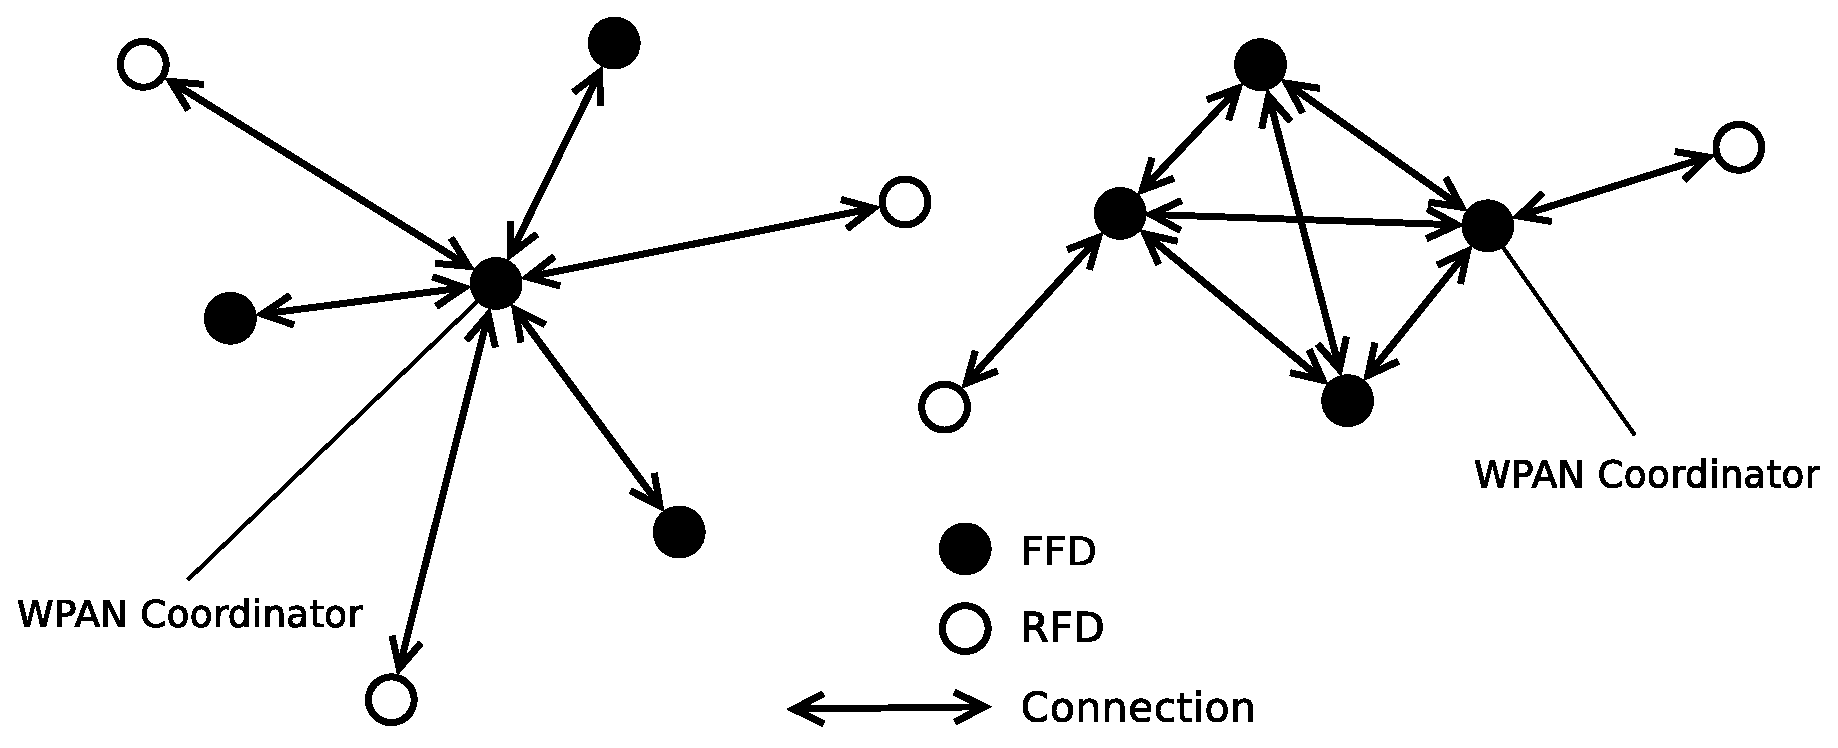
\includegraphics[width=0.9\textwidth]{WPAN_Network_Topologies.eps}
 \end{center}
 \caption{Star and peer-to-peer topology examples \cite{IEEE802.15.4-2006}}
 \label{fig:WPAN_Network_Topologies}
\end{figure}
\end{itemize}
This work will use the peer-to-peer topology as it is more flexible and scalable than the star topology. This topology is also
complexer, that is why a simpler case of peer-to-peer topology is selected, the tree topology. In this case all devices are
structured hierarchically and all of them have a father with whom they communicate, excepting the \ac{WPAN} Coordinator who is on the top of the network.

For making this topology work, a Network Layer (not provided in 802.15.4) is needed for routing purposes. To make packets as short as possible,
and only in communicaton among \acp{FFD}, short addresses (16 bits) will be used.

\section{Physic Layer}

Although for this work \ac{PHY} Layer has not as much importance as the \ac{MAC} Layer, there are some aspects that are important and 
that are good to know. This section will focus just on these aspects.

Some of the tasks developed by the \ac{PHY} Layer are:

\begin{itemize}
 \item \textbf{Switches on and off the radio transceiver.} The transceiver has three operation modes: \ac{Tx}, \ac{Rx} and sleeping. \ac{PHY}
layer must commute among these modes by \ac{MAC} layer petitions. The standard defines that the change time between \ac{Rx} and 
\ac{Tx} and vice versa must not be bigger as 12 symbols (\textit{aTurnaroundTime} = 12 symbols = 192 $\mu$s at 2.4 GHz).
 \item \textbf{Performs the \ac{ED} of the channel.} \ac{PHY} layer measures the power level of the channels in order to choose the best one
to transmit. This measurement lasts exactly 8 symbols.
 \item \textbf{Performs \ac{CCA} to check the channel.} This indicator is a part of \ac{CSMA/CA} algorithm as it will be seen later. The
\ac{CCA} is requested by the \ac{MAC} Layer and the \ac{PHY} Layer returns IDLE or BUSY depending on the channel situation. This \ac{CCA}
period lasts exactly like the \ac{ED}, 8 symbols (128 $\mu$s at 2.4 GHz).
 \item \textbf{Channel frequency selection.} As it was already commented, the 802.15.4 standard contemplates 3 different frequency 
ranges, although only the 2450 MHz will be used in this work. At this frequency, the standard stipulates 
the use of a \ac{O-QPSK} modulation with a symbol rate of 62,5 symbols/s. As this modulation makes 4 bit per symbol, we get 
a 250 Kbit/s bit rate. This frequency range has 16 different channels with a 5 MHz separation between them. The number of 
these channels goes from 11 to 26.
 \item \textbf{Data transmission and reception.} According to the standard, the \ac{PHY} Layer must be able to transmit with a minimum
power of 1 mW and it must have a sensibility of at least -85 dBm \cite{IEEE802.15.4-2006}. Figure \ref{fig:PPDU} shows the physical level frame structure.

\vspace*{1cm}

\begin{figure}[ht]
 \begin{center}
  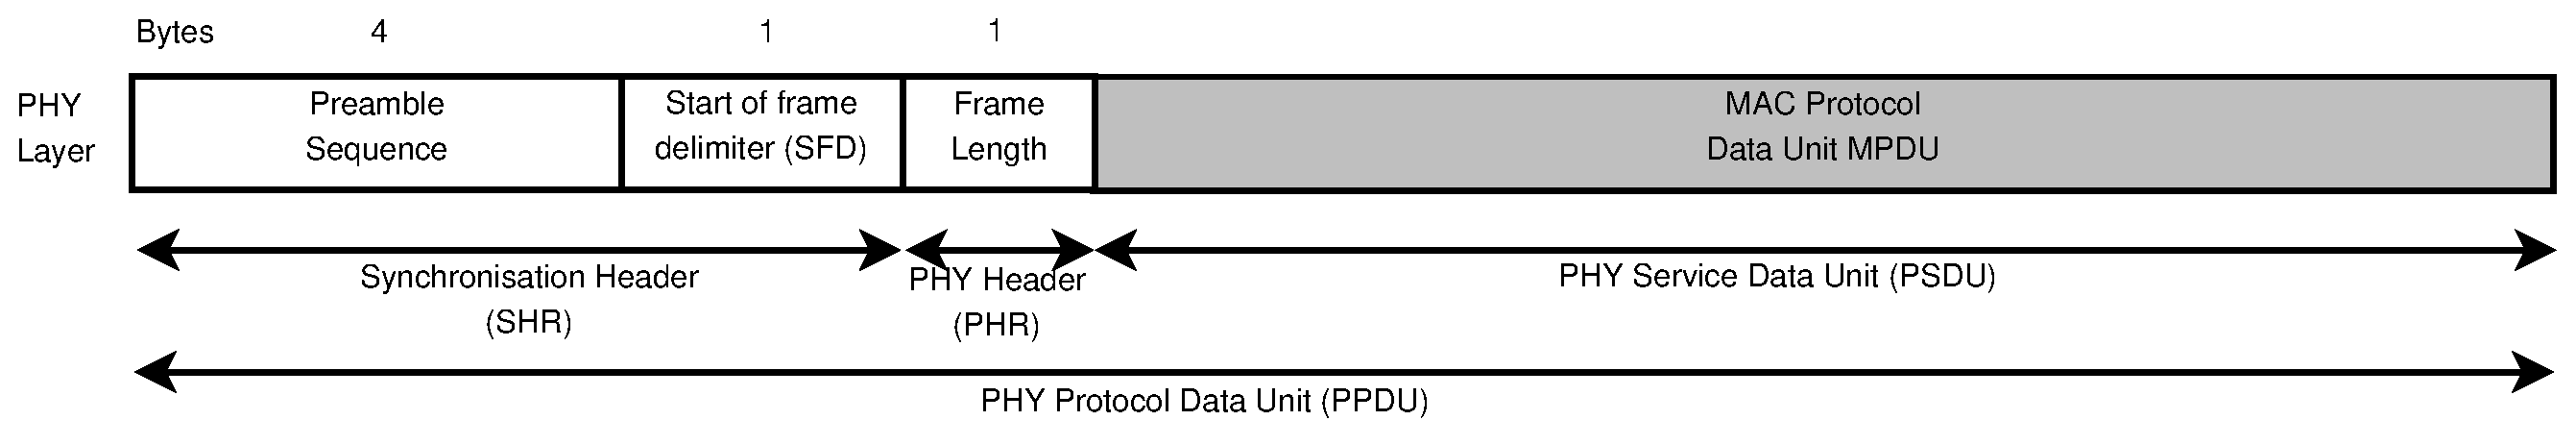
\includegraphics[width=0.9\textwidth]{PPDU.eps}
 \end{center}
 \caption{\ac{PHY} Layer frame \cite{IEEE802.15.4-2006}}
 \label{fig:PPDU}
\end{figure}
\end{itemize}

\section{\ac{MAC} Layer}

\ac{MAC} layer is responsible for connecting the node with all the other nodes in a reachable distance. Although this layer has a reduced
primitive set (26 primitives), it is really versatile and assures the minimum necessary instructions to work. Some of the responsibilities of \ac{MAC}
layer are:

\begin{itemize}
 \item Assures a reliable link between two \ac{MAC} entities.
 \item Beacon generation if device is a router.
 \item Beacon synchronization.
 \item Nodes association and dissociation.
 \item Security mechanisms.
 \item Channel access control through \ac{CSMA/CA}.
 \item Definition of \ac{GTS}.
 \item Frame validation.
 \item Duplicated received packets control.
 \item \ac{ACK} generation to assure retransmission in \ac{MAC} layer. This is a transmission protection mechanism.
\end{itemize}

As happened for the \ac{PHY} layer, the \ac{MAC} layer has some constants and attributes to be configured, which will be used later in this work.
These parameters can be found from page 133 in \cite{IEEE802.15.4-2006}.

\subsection{Working Modes}

\ac{MAC} protocol supports two working modes. The coordinator is the one responsible to choose a mode when initializing the network:

\begin{itemize}
 \item \textbf{Beaconed mode.} In this mode, the coordinator generates a beacon which is transmitted along the network thanks to the routers.
This beacon synchronizes all the devices in the network so they can sleep all the time and just wake up when they know the data will come. 
 \item \textbf{Non-Beaconed mode.} In this mode, the devices are not synchronized by beacons. For this reason, the routers and the coordinator must
be awake all the time and the end devices are the only ones that can sleep. This is not a problem, as we assumed that \ac{FFD} would be plugged 
in and only \ac{RFD} would work with batteries. Furthermore, the problem that end devices do not know when the data from the router will come, 
will be solved with the help of the proposed High Configurable Protocol.
\end{itemize}

Non-Beacon mode was selected for this work as it is more flexible for our purposes than Beaconed mode. The challenge of this choice is to 
define in Application Layer all the sleep and wake-up processes, which would have been automatically administrated in the rejected Beaconed
mode by \ac{MAC} Layer. From now on, all explanations will refer only to Non-Beaconed mode.

\subsection{\ac{CSMA/CA} Algorithm}

When \ac{MAC} Layer receives a message to be sent, before sending it, asks the \ac{PHY} Layer to check if the channel is free. In this case, it 
orders the \ac{PHY} Layer to transmit this message. The whole process is controlled by an algorithm which is called \ac{CSMA/CA}. In this 
case as a non-beaconed mode is used, the \ac{CSMA/CA} algorithm corresponds to the non-slotted one, where the random time a device waits 
before transmitting is not synchronized with the beacons. A graphic approach to this algorithm is given in Figure \ref{fig:CSMACA}, where the
processes to be commented are signaled with a number in brackets.

\begin{itemize}
 \item \textbf{(1)} - Restarts the parameters to their initial values. \ac{NB} is a counter of the number of times the process was done. \ac{BE}
is the exponent for the Backoff Random time calculation. At the beginning it takes the minimum defined by the user (\textit{macMinBE}), usually 3.
 \item \textbf{(2)} - In this step a random number between 0 and $2^{\ac{BE}}$ - 1 is generated and multiplied by the unit Backoff period, defined
by \textit{aUnitBackoffPeriod} in the standard whose default value is 20 symbols = 320 $\mu$s.
 \item \textbf{(3)} - After this waiting period while the node is in IDLE mode, \ac{MAC} orders \ac{PHY} to sense the channel performing the \ac{CCA} 
(8 symbols = 128 $\mu$s). If the channel is free, the \ac{MAC} proceeds to transmit the packet and if not, the algorithm proceeds with the 
step (4).
 \item \textbf{(4)} - If the channel was busy, first \ac{NB} and \ac{BE} are raised in one unit. Afterward, if the new \ac{BE} is bigger than the maximum
(\textit{macMaxBE}), usually 5, \ac{BE} is assigned this maximum value.
 \item \textbf{(5)} - Then maximum number of tries (\textit{macMaxCSMABackOffs}) is checked. If the maximum is not reached, the process starts again from (2),
but if it is reached, the entire process gets canceled and \ac{MAC} layer informs upper layers about the failure (\ac{CAF}).
\end{itemize}

\begin{figure}[!ht]
 \begin{center}
  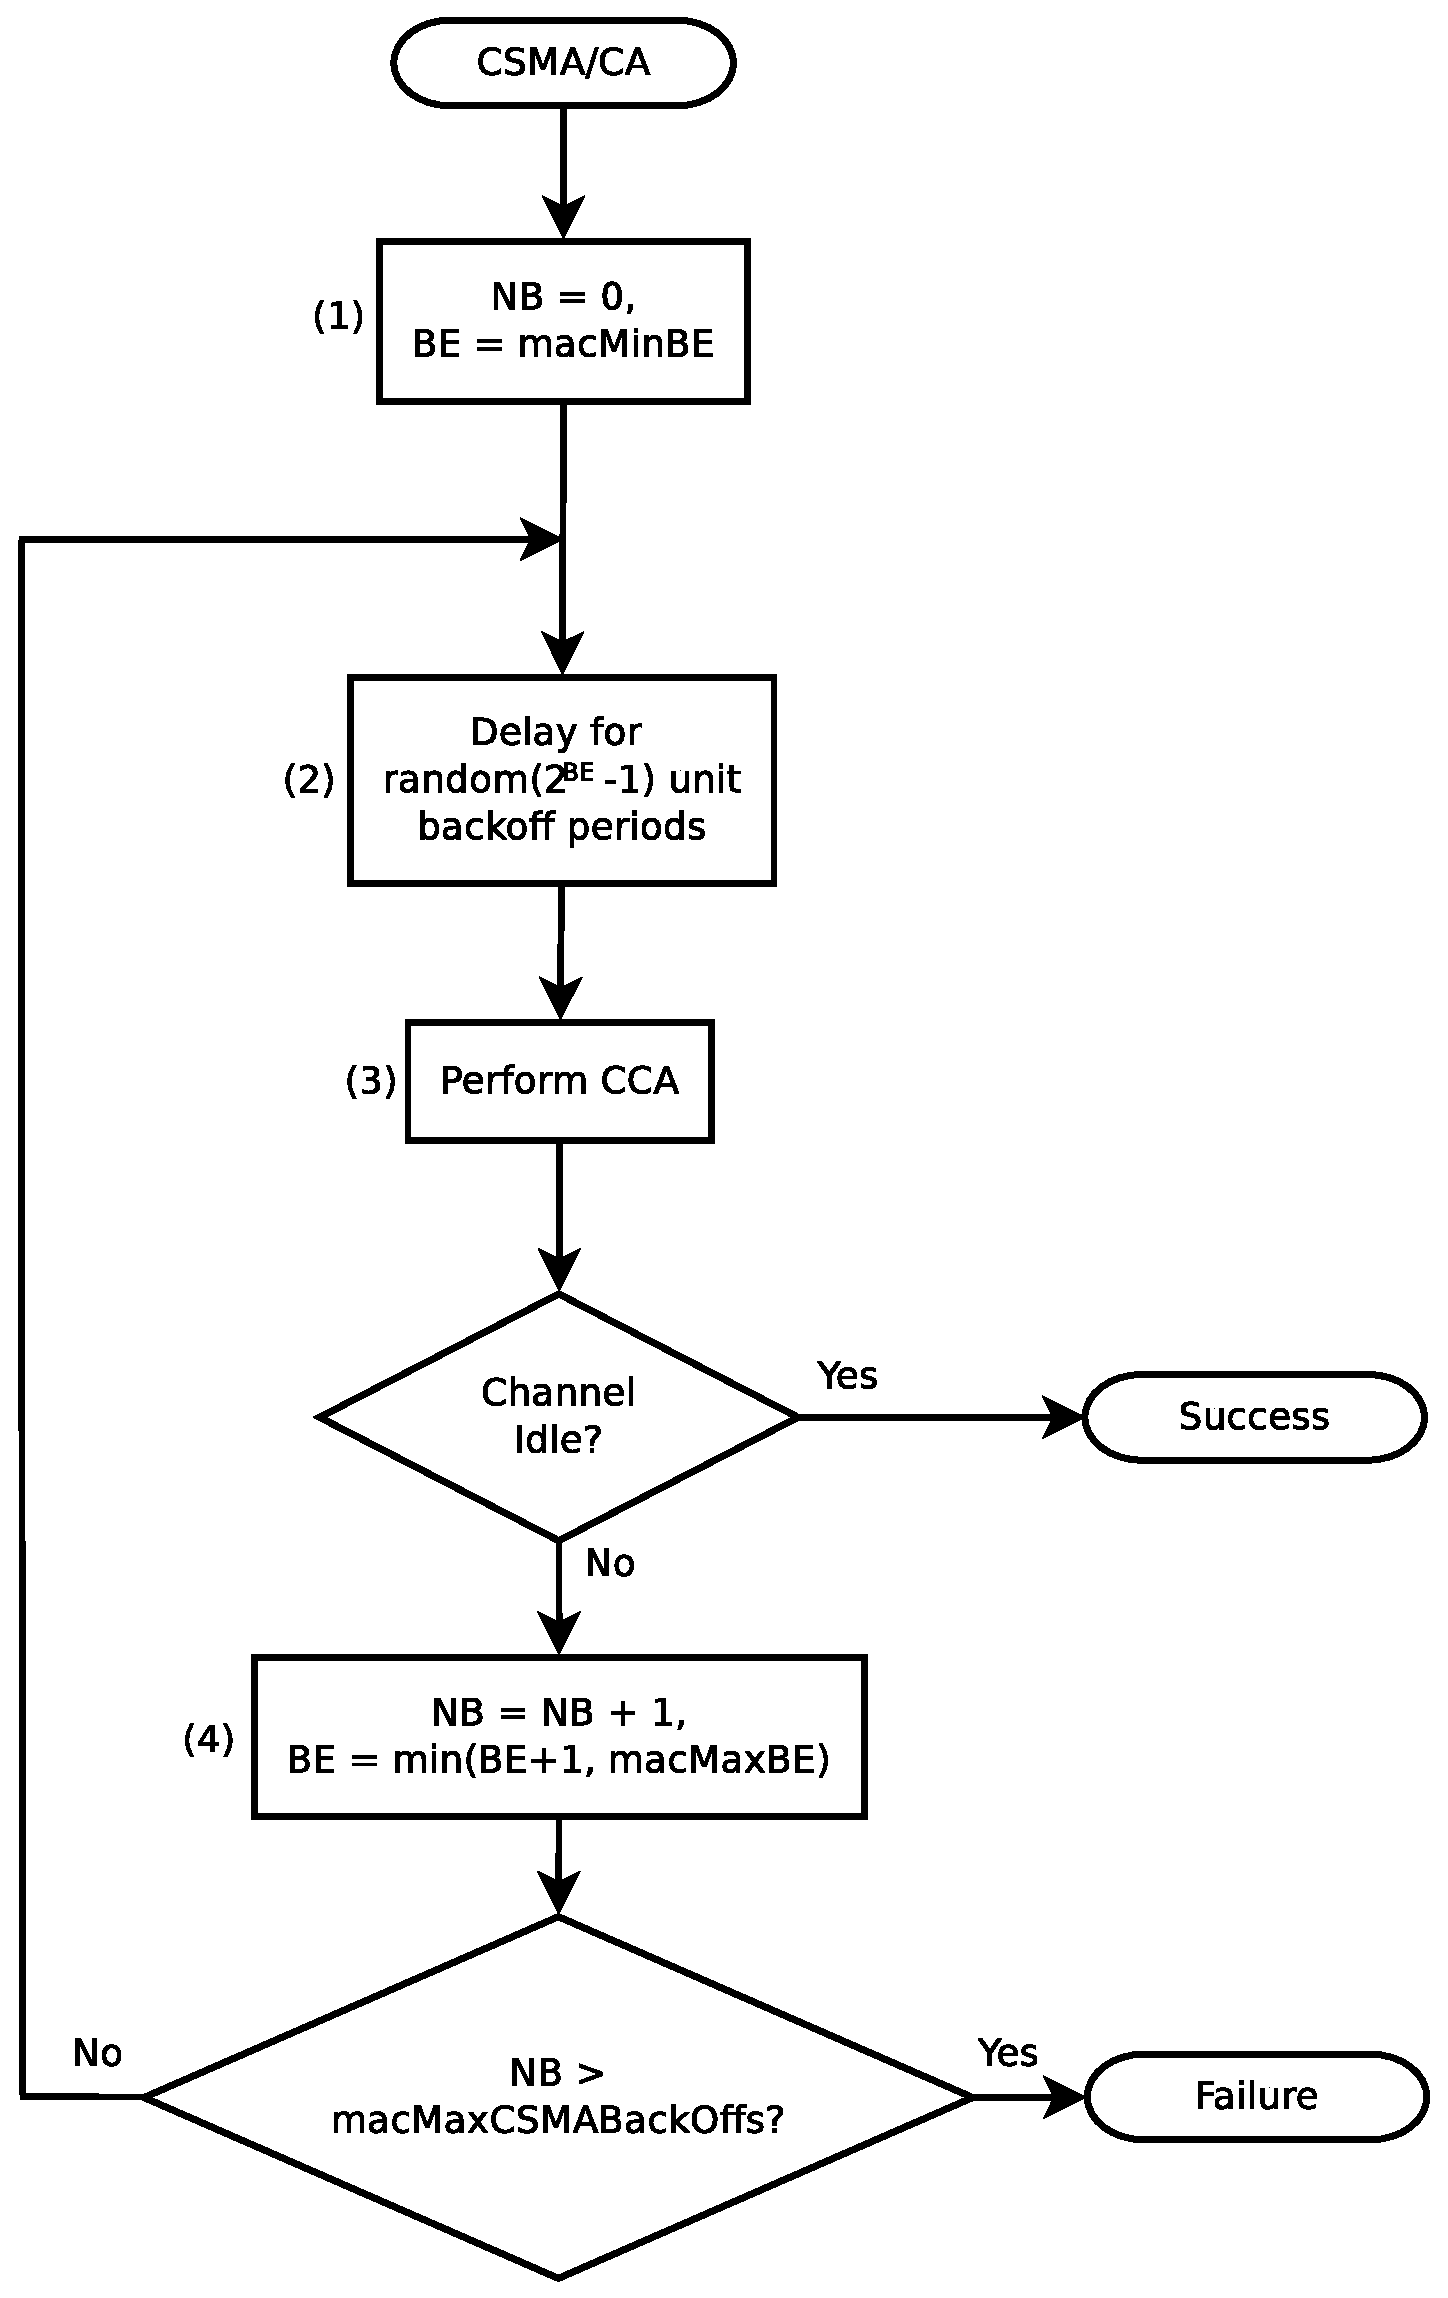
\includegraphics[width=0.5\textwidth]{CSMACA.eps}
 \end{center}
 \caption{Non-Slotted \ac{CSMA/CA} Algorithm \cite{IEEE802.15.4-2006}}
 \label{fig:CSMACA}
\end{figure}

This algorithm helps to reduce the so called collisions. These collisions could occur when a node starts transmitting without checking the 
channel, and if another node next to it has already sent some packet.

But using \ac{CSMA/CA} algorithm does not solve this problem. It could also happen that two packets have a collision in the air. One 
reason could be that while one node is performing the \ac{CCA}, another node does the same. In this case, both of them will start transmitting 
producing a collision. The other reason is the well known Hidden Terminal Problem. To explain this phenomena, Figure \ref{fig:HiddenTerminalProblem}
will be used. Node A wants to communicate with node B, but node C is already transmitting something to node B. As we can see with the dotted line,
the range of A does not cover node C. Because of this, when A performs the \ac{CCA}, it does not get any signal from C. Then node A starts transmitting, and 
node B takes at the same time a message from A and C, having a collision.

\begin{figure}[!ht]
 \begin{center}
  \includegraphics[width=0.3\textwidth]{HiddenTerminalProblem.eps}
 \end{center}
 \caption{Hidden Terminal Problem Scenario}
 \label{fig:HiddenTerminalProblem}
\end{figure}

\ac{CSMA/CA} algorithm makes also possible a situation where a node could transmit without collision but it detects a packet in the air and does
not transmit. To explain this case, Figure \ref{fig:ExposedNodeProblem} will be used. In this situation, C is already transmitting something to D and B 
wants to transmit some information to A. When B performs the \ac{CCA}, it detects the channel as busy with C to D packet. Therefore B waits another
Backoff random time and does not transmit, although it could, as its packet would have reached A and would not have disturbed D.

\begin{figure}[!ht]
 \begin{center}
  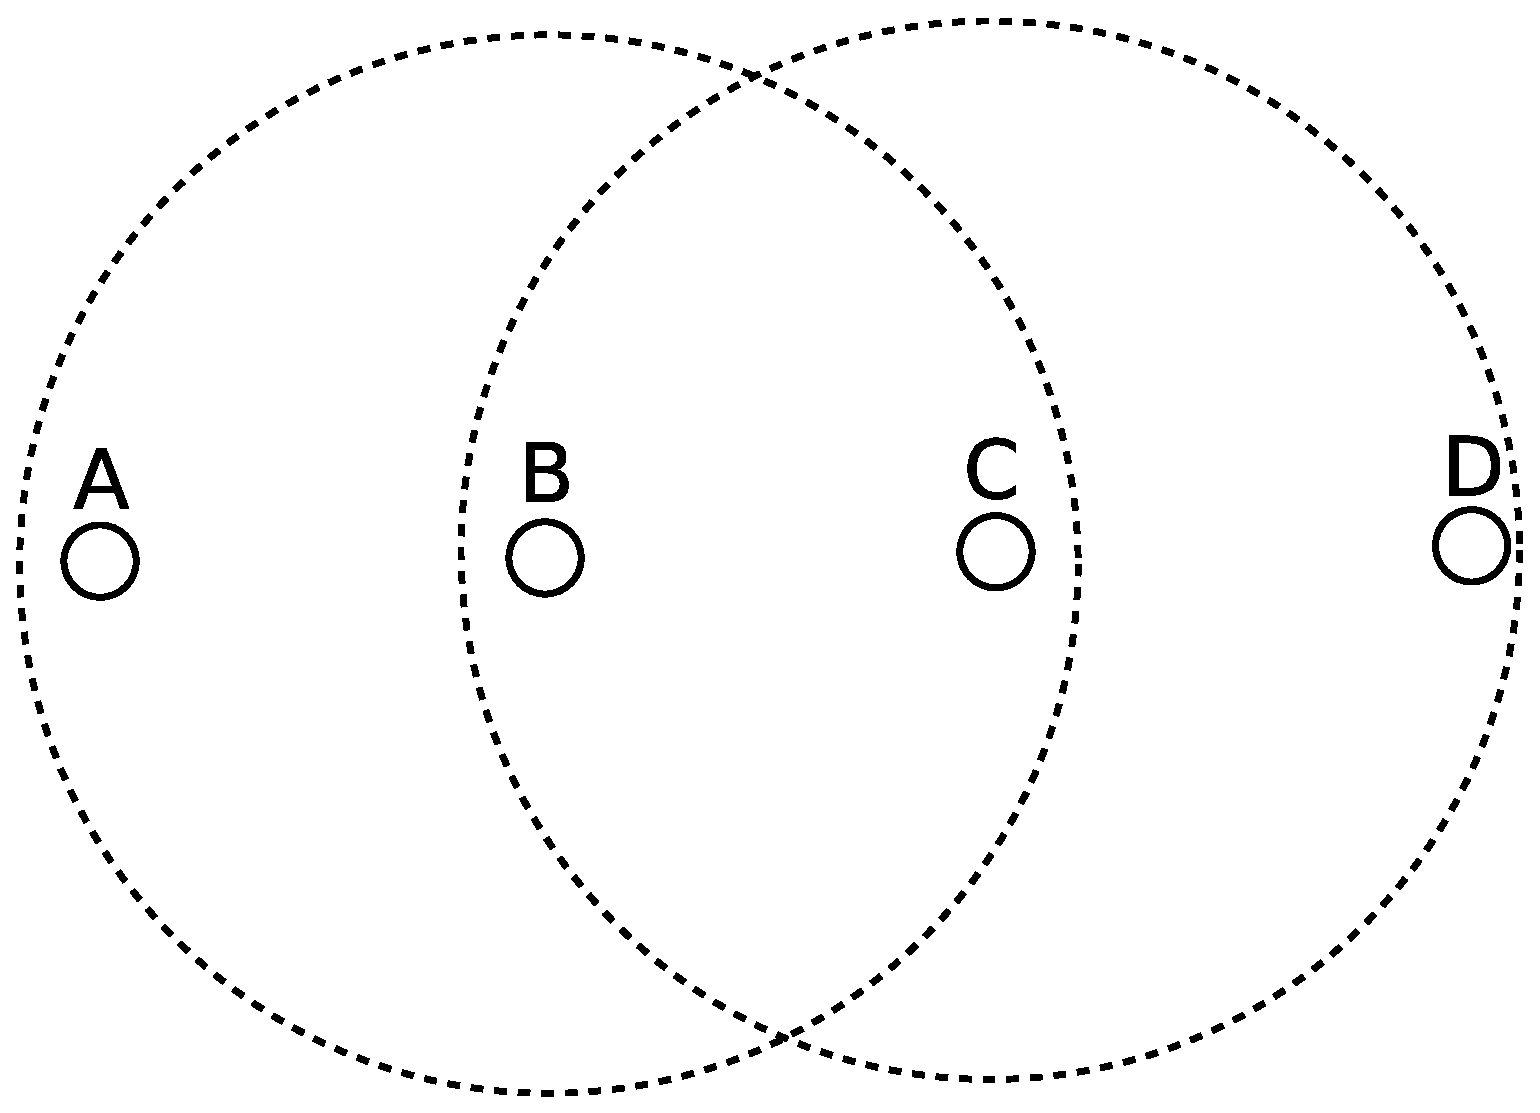
\includegraphics[width=0.3\textwidth]{ExposedNodeProblem.eps}
 \end{center}
 \caption{Exposed Node Problem Scenario}
 \label{fig:ExposedNodeProblem}
\end{figure}

Apart from the times already commented like \ac{CCA} or Backoff, there are other important times to be taken into account. \ac{SIFS} is the 
time to leave between two consecutive frames when the frame was short $(\le 18 bytes)$ and its value is 12 symbols = 192 $\mu$s. \ac{LIFS} 
is the same as \ac{SIFS} but to use with long frames (40 symbols = 640 $\mu$s). Usually these two times are included in \ac{CSMA/CA} process, 
and they are important not to collapse the system and lose data. Another important time is \textit{aTurnaroundTime}, this time is 192 $\mu$s 
and corresponds to the time needed to switch between \ac{Rx} and \ac{Tx} modes and vice versa. It is also the time to leave between the end 
of a packet reception and the start of the \ac{ACK} transmission.

\subsection{Frame Format}

\ac{MAC} packets use different frames depending if the network is beaconed or non-beaconed. As this work is using just the non-beaconed mode,
only the frames related to this mode will be explained. Figure \ref{fig:MACFrame} contains the structure that will be explained now.

\begin{figure}[!ht]
 \begin{center}
  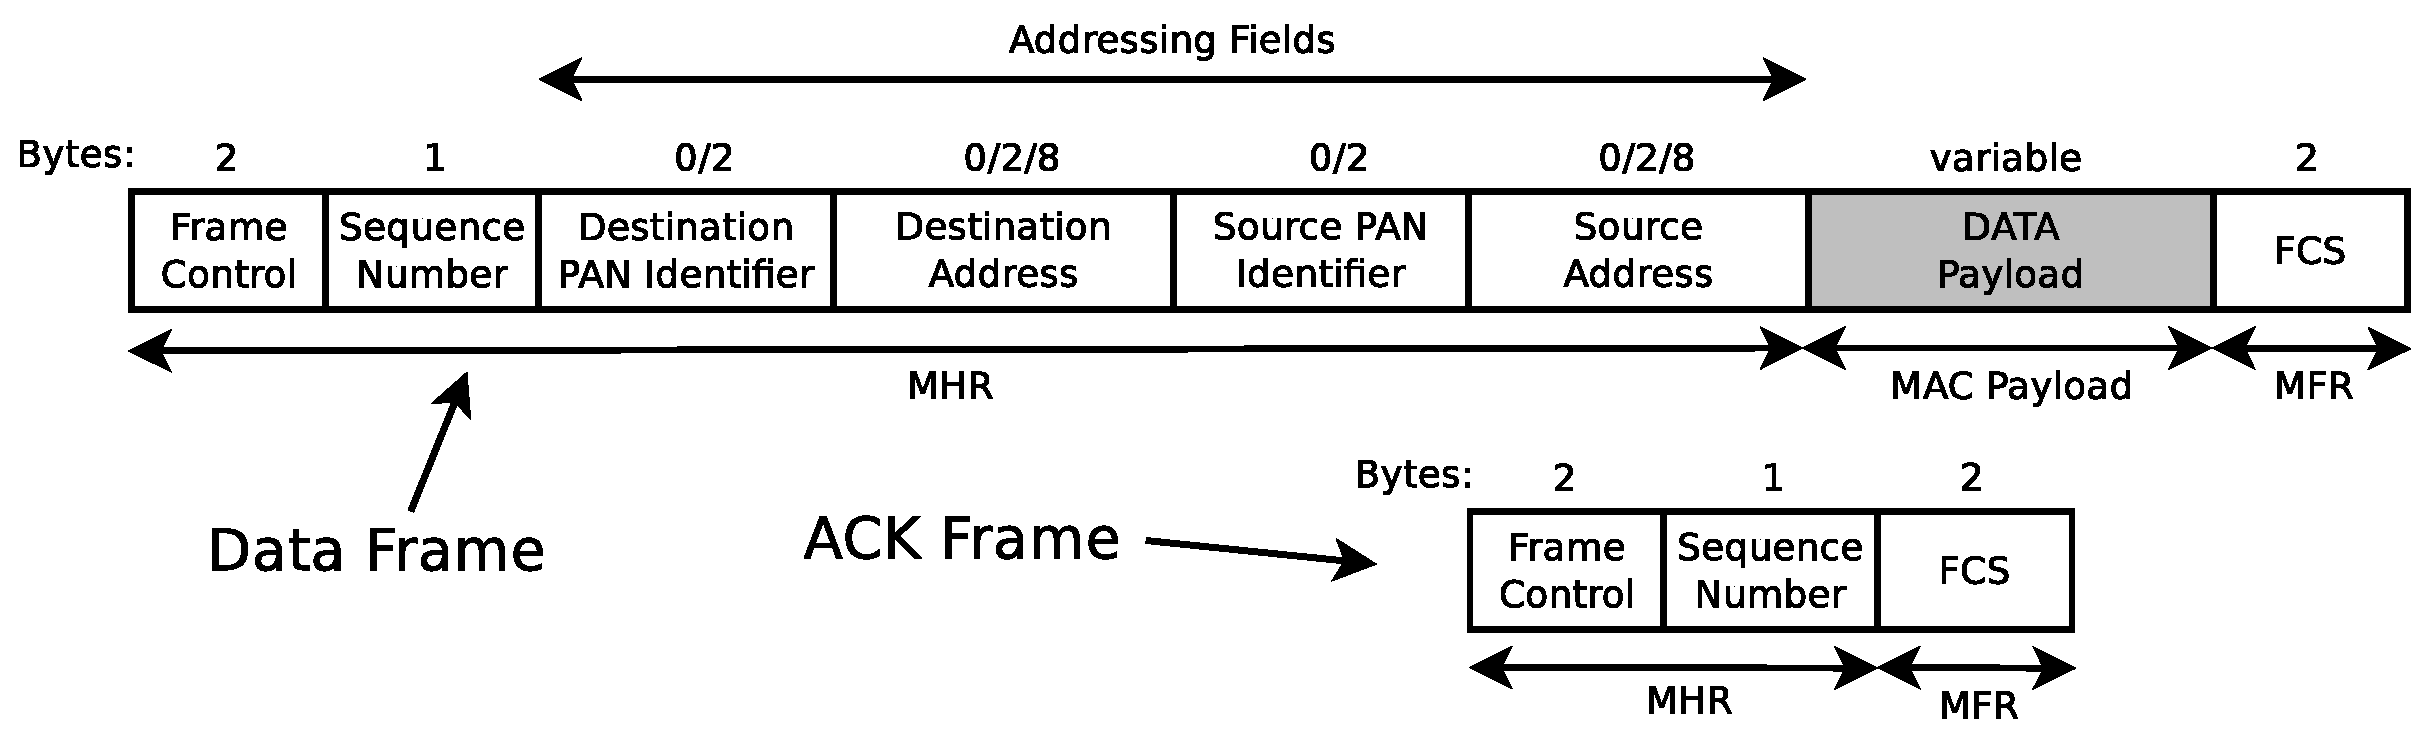
\includegraphics[width=0.7\textwidth]{MACFrame.eps}
 \end{center}
 \caption{Data and \ac{ACK} \ac{MAC} Frames \cite{IEEE802.15.4-2006}}
 \label{fig:MACFrame}
\end{figure}

\begin{itemize}
 \item \textbf{Header (\ac{MHR}).} Formed by:
  \begin{itemize}
   \item Frame Control: 16 bits to define the frame type, security code, \ac{ACK} required, etc.
   \item Sequence Number: 8 bits to identify the frame.
   \item Destination \ac{PAN} Identifier: 16 bits to indicate the \ac{PAN} communicating with. 0xFFFF if any network is selected.
   \item Destination Address: 16 or 64 bits depending if it is a short or long address. End devices use always a long address and routers a short one.
   \item Source PAN Identifier: 16 bits to indicate the source \ac{PAN}.
   \item Source Address: 16 or 64 bits depending if it is a short or long address, end devices use always long address and routers short.
  \end{itemize}
 \item \textbf{Payload.} Data from upper layer.
 \item \textbf{\ac{MFR}.} 16 bit sequence known as \ac{FCS}, this is a \ac{CRC}.
\end{itemize}

\subsection{Hardware}

Although this work is based on a simulation, all the needed physical parameters to simulate are obtained from the commercial hardware 
RCB230 V3.2 as it is the one available in the department. This node has a AT86RF230 transceiver and a ATmega1281V \ac{uC}. According 
to \cite{LPLandOLP}, the consumption values of this node are the ones shown in Table \ref{tab:NodeEnergyConsumption}. Transition times that are not defined
in 802.15.4 standard are in Table \ref{tab:NodeTiming}.


\begin{table}
 \begin{center}
  \begin{tabular}{|l|c|}
   %\noalign{\vspace*{0.5cm}}
   \hline
   & \textbf{Energy Consumption} \\
   \hline
   Transceiver \ac{Rx} mode & 0.06496 mW/s \\
   \hline 
   Transceiver \ac{Tx} mode & 0.06672 mW/s \\
   \hline
   Transceiver IDLE mode & 0.04342 mW/s \\
   \hline
   Transceiver Sleep mode & 0.0728 $\mu$W/s \\
   \hline
   \ac{uC} (Transceiver Sleeps) & 0.03042 mW/s \\
   \hline
  \end{tabular}
  \caption{Node RCB230 V3.2 Energy Consumption \cite{LPLandOLP}}
  \label{tab:NodeEnergyConsumption}
 \end{center}
\end{table}
\begin{table}
 \begin{center}
  \begin{tabular}{|l|c|}
   %\noalign{\vspace*{0.5cm}}
   \hline
   & \textbf{Transition timing} \\
   \hline
   Transition: Sleep -> \ac{Rx} & 1.88 ms \\
   \hline 
   Transition: \ac{Tx} -> Sleep & 0.94 ms \\
   \hline
   Transition: \ac{Rx} -> Sleep & 0.94 ms \\
   \hline
  \end{tabular}
  \caption{Transceiver AT86RF230 transition timing \cite{LPLandOLP}}
  \label{tab:NodeTiming}
 \end{center}
\end{table}

